\documentclass[twoside]{article}

\usepackage{aistats2027}
% For the camera-ready version, use:
% \usepackage[accepted]{aistats2027}

\usepackage[round]{natbib}
\renewcommand{\bibname}{References}
\renewcommand{\bibsection}{\subsubsection*{\bibname}}
\bibliographystyle{apalike}

\usepackage[utf8]{inputenc}
\usepackage{amsmath,amssymb,bm}
\usepackage{booktabs}
\usepackage{xcolor}
\usepackage{tikz}
\usetikzlibrary{arrows.meta,positioning,calc}
\usepackage[hidelinks]{hyperref}
\hyphenation{can-di-date-in-de-pen-dent}

\newcommand{\ours}{ECHO}
\newcommand{\R}{\mathbb{R}}
\newcommand{\first}[1]{\textbf{#1}}
\newcommand{\second}[1]{\underline{#1}}
\newcommand{\lone}{\operatorname{lg}}
% placeholder for numbers that still have to be measured; renders in red so that none is left by accident
\newcommand{\tbd}[1][TBD]{\textcolor{red}{[#1]}}

\begin{document}

\runningtitle{ECHO: Reading Evidence Beyond the History Window for Future Link Prediction}

\twocolumn[

\aistatstitle{ECHO: Reading Evidence Beyond the History Window\\ for Future Link Prediction on Temporal Graphs}

\aistatsauthor{ Author 1 \And Author 2 \And Author 3 }

\aistatsaddress{ Institution 1 \And Institution 2 \And Institution 3 } ]

\begin{abstract}
State-of-the-art models for future link prediction on temporal graphs score each candidate destination against a bounded, undirected window of the source's own most recent interactions. We show that a substantial share of future links is explained by evidence that lies outside this window. In directed graphs, the window does not record who initiated each past interaction, yet on uci 64\% of new edges answer an earlier edge in the opposite direction. In long histories, the window truncates the past: on lastfm, 25.5\% of edges return to an item the user interacted with before, but outside the window. When the source has never met the candidate, its own history holds no evidence at all: on GoogleLocal, 58.8\% of true destinations are co-visited with the source's history by other users, against 1.9\% of random candidates. We propose Explicit Closure and History Observations (\ours{}), which exposes this evidence to a target-aware matching backbone through three readouts (reciprocity, long-range memory, and co-visit closure) computed by binary searches on time-sorted event indexes. \ours{} samples no additional neighbors, counts only events strictly before the prediction time, and enters the model through a gated correction that starts at zero. On eight benchmarks, \ours{} improves the mean MRR of CRAFT on every dataset, by up to 10.64 points, and the gains follow the measured properties of each dataset.
\end{abstract}

\section{Introduction}

Dynamic systems are typically formulated as temporal graphs, where nodes and edges represent entities and their interactions, and each edge is annotated with a timestamp \citep{kazemi2020representation,fard2023machine,zheng2024survey}. Predicting future interactions between entities is known as future link prediction \citep{divakaran2020temporal}, which is crucial in applications such as social networks \citep{daud2020applications,haghani2019systemic}, collaboration platforms \citep{sun2011coauthor}, and financial systems \citep{rajput2022temporal}. Future interactions can be repeated interactions with historical neighbors (seen edges) or new interactions with previously unconnected nodes (unseen edges) \citep{yi2025tgbseq}, and a practical model must handle both.

The recent CRAFT model \citep{yi2025craft} shows that two ingredients go a long way on both kinds of edges: learnable node embeddings, and target-aware matching, in which each candidate destination attends over the source's $k$ most recent neighbors. Like most temporal graph models, however, CRAFT scores a candidate from a specific slice of the past. The slice is \emph{bounded} (the last $k$ neighbors), \emph{undirected} (the neighbor samplers symmetrize the graph), and \emph{ego-centric} (it contains only the source's own interactions). This paper asks how much of the signal for future links lies outside that slice, and whether it can be read at little cost.

We find that the answer depends on the dataset, but is often large, and that it can be measured before any model is trained (Section~\ref{sec:evidence}). Three kinds of evidence are missing:
\begin{itemize}
\item \textbf{Direction.} The window records that $s$ and $d$ interacted, but not who initiated it, so it cannot tell ``$d$ contacted me and I have not answered'' from ``I contacted $d$''. On uci, 64.0\% of validation edges answer an earlier edge in the opposite direction.
\item \textbf{Older interactions.} On lastfm, the window holds 120 interactions, and 25.5\% of validation edges go to an item that the user interacted with before, but outside the window. For these edges, the backbone's repeat count is zero and its attention finds no match.
\item \textbf{Other users.} When the source has never met the candidate, its own history contains no direct evidence. GoogleLocal has no repeated edges, and its median user has 5 interactions. Yet 58.8\% of its validation positives are \emph{co-visited} with the source's history by another user, against 1.9\% of random candidates.
\end{itemize}

These are classic signals: reciprocity drives point-process models of communication \citep{blundell2012modelling}, repeated consumption underlies memorization baselines \citep{poursafaei2022towards}, and co-visits are the basis of item-based collaborative filtering \citep{sarwar2001item}. The difficulty is not to know that they matter, but to provide them to a target-aware model without paying for it. Widening the window increases the cost of attention linearly in $k$ and still records neither direction nor other users, while sampling the neighbors of every candidate, as structural encoders do, multiplies the sampling cost by the number of candidates \citep{yi2025craft}.

We propose Explicit Closure and History Observations (\ours{}), which keeps target-aware matching as the backbone and adds three readouts of the missing evidence. All events are indexed once, sorted by key and time, so that every statistic is a difference of binary searches. \ours{} samples no additional neighbors, counts only events strictly before the prediction time, and adds its readouts to the backbone logit through a gate that starts at zero. Our contributions are:
\begin{itemize}
\item A measurement of the evidence that lies outside the bounded, undirected, ego-centric window of target-aware matching, on the validation splits of standard benchmarks.
\item \ours{}, which reads this evidence from time-sorted indexes with $O(\log P)$ queries, without additional neighbor sampling and without leakage across time or splits.
\item Experiments on eight benchmarks, where \ours{} improves the mean MRR of CRAFT on every dataset, by up to 10.64 points, and where the size of the gain follows the measured properties of each dataset.
\end{itemize}

\section{Related Work}

\textbf{Temporal graph learning for future link prediction.}
Most methods adopt one or both of the memory and aggregation modules \citep{skarding2021foundations,rossi2020tgn,yang2024towards}. JODIE \citep{kumar2019jodie}, DyRep \citep{trivedi2019dyrep}, and TGN \citep{rossi2020tgn} update node memory with RNNs \citep{wu2017recurrent} or GRUs \citep{cho2014learning}, while TGAT \citep{xu2020tgat}, CAWN \citep{wang2021cawn}, GraphMixer \citep{cong2023graphmixer}, TCL \citep{wang2021tcl}, SimpleDyG \citep{wu2024simpledyg}, and DyGFormer \citep{yu2023dygformer} aggregate historical neighbors with attention, random walks, or the MLP-Mixer \citep{tolstikhin2021mlp}. Other methods use temporal point processes \citep{hawkes1971spectra,mei2017neural}, such as TREND \citep{wen2022trend} and LDG \citep{knyazev2021learning}. CRAFT \citep{yi2025craft} discards memory and aggregation and performs target-aware matching over learnable node embeddings \citep{abboud2020surprising,loukas2019graph,bechler2025towards}. \ours{} keeps this backbone and changes what it can observe.

\textbf{Pairwise structure between source and destination.}
Several methods encode how the neighborhoods of the two endpoints relate. CAWN \citep{wang2021cawn} uses anonymous walks, NAT \citep{luo2022neighborhood} maintains neighborhood dictionaries, DyGFormer \citep{yu2023dygformer} and FreeDyG \citep{tian2024freedyg} encode neighbor co-occurrence and interaction frequencies, TNCN \citep{zhang2024tncn} extends neural common neighbors to temporal graphs, TPNet \citep{lu2024tpnet} projects time-decayed temporal walk matrices, and HOT \citep{besta2024hot} models higher-order structures. Most of these methods compute the structure from sampled neighbors of both endpoints of every candidate edge. \ours{} reads a small set of pair, node, and co-visit counts from indexes keyed by node pairs. The co-visit readout reaches two hops from the source without sampling the candidate's neighbors.

\textbf{Reciprocity, repetition, and co-visits.}
Reciprocating relationships are a central object of point-process models of interaction data \citep{blundell2012modelling}. Memorization of past pairs is a strong baseline on seen-dominant data \citep{poursafaei2022towards}, and item-to-item co-occurrence is the basis of item-based collaborative filtering \citep{sarwar2001item}. Sequential recommenders such as SASRec \citep{kang2018sasrec} and SGNN-HN \citep{pan2020sgnnhn} are strong on the unseen-dominant TGB-Seq benchmark \citep{yi2025tgbseq}. \ours{} does not propose these signals. It computes them causally on a temporal graph and makes them available to a target-aware model at logarithmic cost.

\section{Problem Formulation}

\textbf{Temporal graphs.} A temporal graph is $\mathcal{G}=(\mathcal{V},\mathcal{E})$, where $\mathcal{V}$ is a set of nodes and $\mathcal{E}=\{e_1,\cdots,e_m\}$ is a sequence of edges with non-decreasing timestamps, each edge $e_i=(s_i,d_i,t_i)$ denoting an interaction from the source $s_i$ to the destination $d_i$ at time $t_i$.

\textbf{Future link prediction.} Given all edges before time $t$, future link prediction estimates the likelihood of an interaction between a source $s$ and a destination $d$ at time $t$. Following prior work \citep{huang2024tgb,yi2025tgbseq,yi2025craft}, we frame it as ranking the positive destination above sampled negative candidates, conditioned on $s$ and $t$.

\section{Evidence Beyond the History Window}
\label{sec:evidence}

Target-aware matching scores a candidate $d$ from the source's $k$ most recent neighbors, sampled from a symmetrized graph. We measure, for each validation edge $(s,d,t)$, three properties that this window cannot express. All statistics use only events strictly before $t$; co-visits are counted on the training split only, so no test data is involved. Appendix~\ref{app:stats} gives the exact definitions.

\begin{itemize}
\item \textbf{Reply rate}: the share of edges $s\to d$ such that $d\to s$ occurred earlier. It is zero on bipartite graphs.
\item \textbf{Repeats in and beyond the window}: the share of edges whose destination is among the $k$ most recent neighbors of $s$, and the share whose destination is an earlier neighbor of $s$ outside them.
\item \textbf{Co-visit closure}: the share of edges whose destination was interacted with by some user $u\neq s$ within $\omega=20$ interactions of an item in the window of $s$. We compare positives with uniformly random candidates.
\end{itemize}

\begin{table}[t]
\caption{Evidence outside the window of target-aware matching, on validation edges (\%). $k$ is CRAFT's window on each dataset. Co-visit closure is reported for positives / random candidates.}
\label{tab:evidence}
\begin{center}
\resizebox{\columnwidth}{!}{%
\setlength{\tabcolsep}{3pt}
\begin{tabular}{lrrrrr}
\toprule
Dataset & $k$ & Reply & In win. & Beyond & Co-visit (pos/rnd) \\
\midrule
uci & 30 & 64.0 & 70.8 & 4.7 & 63.8 / 50.4 \\
mooc & 30 & 0 & 53.6 & 5.1 & 99.4 / 95.1 \\
lastfm & 120 & 0 & 64.6 & 25.5 & 95.1 / 99.4 \\
GoogleLocal & 60 & 0 & 0 & 0 & 58.8 / \phantom{0}1.9 \\
\midrule
Flickr & \tbd & \tbd & 0 & 0 & \tbd \\
YouTube & \tbd & \tbd & 0 & 0 & \tbd \\
wikipedia & 120 & 0 & \tbd & \tbd & \tbd \\
reddit & 120 & 0 & \tbd & \tbd & \tbd \\
\bottomrule
\end{tabular}}
\end{center}
\end{table}

Table~\ref{tab:evidence} shows that the missing evidence differs across datasets, and that each dataset is dominated by a different kind. On uci, most new edges are replies. On lastfm, a quarter of the edges return to an item that has left the window. On GoogleLocal, nothing is repeated and the window offers no match, but co-visits separate the positives from random candidates by a factor of 30. On mooc, little evidence is missing: few repeats leave the window, and with only 97 destinations nearly every candidate is co-visited with the history, so co-visits do not separate positives from negatives. The same is true of lastfm, whose 1,000 items are densely co-visited. These differences lead to the predictions that we test in Section~\ref{sec:experiments}: \ours{} should gain most on directed graphs with many replies, then on datasets with many repeats beyond the window or with selective co-visits, and least on mooc.

\section{Proposed Method}

\ours{} consists of a target-aware matching backbone (Section~\ref{sec:backbone}), three readouts that correspond to the three kinds of evidence (Sections~\ref{sec:recip}--\ref{sec:covisit}), and a gated fusion (Section~\ref{sec:fusion}). Figure~\ref{fig:arch} shows the architecture. Throughout, $\lone(x)=\log(1+x)$, and $\bar{\tau}$ is a running scale of elapsed times that adapts the time unit to each dataset (Section~\ref{sec:fusion}).

\begin{figure}[t]
\centering
\resizebox{\columnwidth}{!}{%
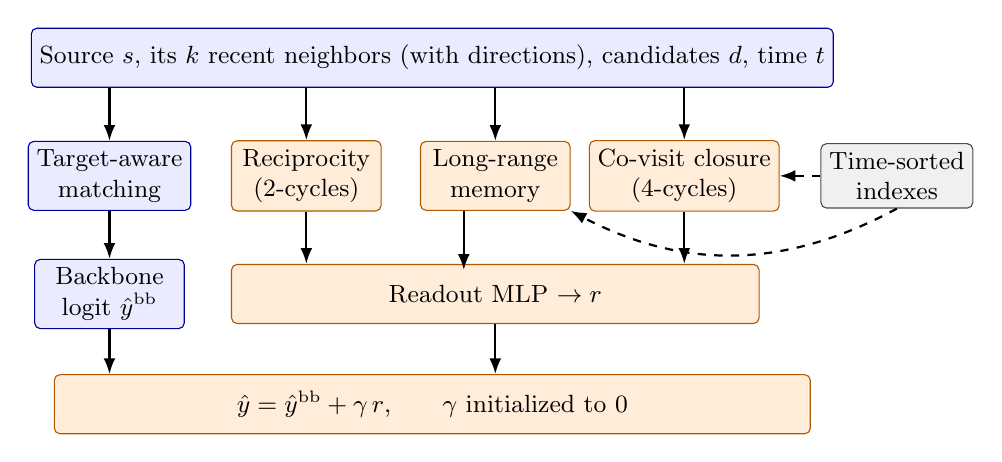
\begin{tikzpicture}[
  font=\small,
  box/.style={draw, rounded corners=2pt, minimum height=0.75cm, align=center, inner sep=3pt},
  new/.style={box, fill=orange!15, draw=orange!70!black},
  old/.style={box, fill=blue!8, draw=blue!60!black},
  idx/.style={box, fill=gray!12, draw=gray!60!black},
  arr/.style={-{Latex[length=2mm]}, thick}
]
\node[old, minimum width=9.6cm] (in) at (4.1,0) {Source $s$, its $k$ recent neighbors (with directions), candidates $d$, time $t$};
\node[old, minimum width=1.9cm] (bb) at (0,-1.5) {Target-aware\\ matching};
\node[new, minimum width=1.9cm] (rec) at (2.5,-1.5) {Reciprocity\\ (2-cycles)};
\node[new, minimum width=1.9cm] (mem) at (4.9,-1.5) {Long-range\\ memory};
\node[new, minimum width=1.9cm] (cov) at (7.3,-1.5) {Co-visit closure\\ (4-cycles)};
\node[idx] (ix) at (10.0,-1.5) {Time-sorted\\ indexes};
\node[old, minimum width=1.9cm] (y0) at (0,-3.0) {Backbone\\ logit $\hat{y}^{\mathrm{bb}}$};
\node[new, minimum width=6.7cm] (mlp) at (4.9,-3.0) {Readout MLP $\rightarrow r$};
\node[new, minimum width=9.6cm] (out) at (4.1,-4.4) {$\hat{y}=\hat{y}^{\mathrm{bb}}+\gamma\, r$,\qquad $\gamma$ initialized to $0$};
\foreach \n in {bb,rec,mem,cov} \draw[arr] (in.south -| \n) -- (\n);
\draw[arr, dashed] (ix) -- (cov);
\draw[arr, dashed] (ix.south) to[bend left=28] (mem.south east);
\draw[arr] (bb) -- (y0);
\foreach \n in {rec,cov} \draw[arr] (\n) -- (\n |- mlp.north);
\draw[arr] (mem.south) ++(-0.4,0) -- ++(0,-0.75);
\draw[arr] (y0) -- (y0 |- out.north);
\draw[arr] (mlp) -- (mlp |- out.north);
\end{tikzpicture}}
\caption{Architecture of \ours{}. Blue blocks form the target-aware matching backbone, which is unchanged; orange blocks are added by \ours{}. The readouts query time-sorted indexes (dashed) with binary searches and sample no additional neighbors.}
\label{fig:arch}
\end{figure}

\subsection{Target-aware Matching Backbone}
\label{sec:backbone}

Given the source $s$ and candidates $\{d_1,\cdots,d_q\}$ at time $t$, we extract the $k$ most recent neighbors $(n_1,\cdots,n_k)$ of $s$ before $t$, with interaction times $(t_1,\cdots,t_k)$. Following CRAFT \citep{yi2025craft}, each node has a learnable embedding $e(n)\in\R^{F}$, and a learnable positional encoding $p(l)$ is added to the $l$-th neighbor. Each candidate is the query of cross-attention layers \citep{vaswani2017attention} over the neighbor sequence. The output is concatenated with a projection of the elapsed time since the candidate's last activity and, on seen-dominant datasets, a projection of the repeat count of the candidate in the window. An MLP maps the result to the backbone logit $\hat{y}^{\mathrm{bb}}_j$ of candidate $d_j$. We use this backbone, and its per-dataset hyperparameters, unchanged.

\subsection{Reciprocity Readout: Direction}
\label{sec:recip}

On directed graphs, the shortest cycle that a new edge $s\to d$ can close is the 2-cycle $d\to s\to d$: a reply or a follow-back. The neighbor sampler returns the identifier of the edge behind each history entry, from which we recover whether $s$ sent it ($\delta_l=1$) or received it ($\delta_l=0$). Let $m_{jl}=\mathbf{1}[n_l=d_j]$ indicate that the $l$-th entry is an interaction with $d_j$, and $\Delta_l=(t-t_l)/\bar{\tau}$ its normalized elapsed time. For each direction $o\in\{0,1\}$,
\begin{equation}
\begin{aligned}
c^{o}_j&=\textstyle\sum_{l}m_{jl}\mathbf{1}[\delta_l=o],\qquad x^{o}_j=\mathbf{1}[c^{o}_j>0],\\
a^{o}_j&=x^{o}_j\cdot\min_{l:\,m_{jl}=1,\,\delta_l=o}\Delta_l,
\end{aligned}
\end{equation}
and $\phi^{\mathrm{rec}}_j=[\lone(a^{o}_j),x^{o}_j,\lone(c^{o}_j)]_{o\in\{0,1\}}\in\R^{6}$. The received half ($o=0$) separates an unanswered incoming interaction from an outgoing one. On bipartite graphs it is zero, and the readout reduces to direction-free recency and counts within the window.

\subsection{Long-range Memory Readout: Older Interactions}
\label{sec:memory}

To remove the bound of the window, we index all past events twice, once keyed by the pair $(s,d)$ and once by the node $d$, each sorted by key and time. For any key, the number of events in $[t_a,t)$ is the difference of two binary searches, whatever the length of the history. Given window multiples $w_1<\cdots<w_W$, we compute for the pair $(s,d_j)$ the counts $N^{\mathrm{pair}}_{j,w}$ in $[t-w\bar{\tau},t)$, the total $N^{\mathrm{pair}}_j$ before $t$, the indicator $x_j=\mathbf{1}[N^{\mathrm{pair}}_j>0]$, and the normalized time $\rho_j$ since the latest occurrence. For the node $d_j$, we compute the windowed counts $N^{\mathrm{node}}_{j,w}$ and the total $N^{\mathrm{node}}_j$, which describe the candidate's recent and overall popularity. The readout is
\begin{equation}
\begin{aligned}
\phi^{\mathrm{mem}}_j=\big[&\lone(N^{\mathrm{pair}}_{j,w})_{w},\ \lone(N^{\mathrm{pair}}_j),\ x_j,\ \lone(\rho_j),\\
&\lone(N^{\mathrm{node}}_{j,w})_{w},\ \lone(N^{\mathrm{node}}_j)\big],
\end{aligned}
\end{equation}
with $2W+4$ dimensions. Because the windows are multiples of $\bar{\tau}$, the same multiples serve datasets with different time units.

\subsection{Co-visit Closure Readout: Other Users}
\label{sec:covisit}

For a candidate that the source has never met, the shortest cycle in a bipartite graph is the 4-cycle $s - i - u - d$: another node $u$ interacted with an item $i$ that $s$ visited, and also with $d$. A co-visit of $(i,d)$ is a node $u$ interacting with both $i$ and $d$ within $\omega$ consecutive interactions of $u$, timestamped at the later of the two. Co-visits are indexed by the unordered pair $\{i,d\}$ and sorted by time, so that their number before $t$ is again a difference of binary searches. For each history item $n_l$ and candidate $d_j$, let $c_{jl}$ be the number of co-visits of $(n_l,d_j)$ before $t$, and
\begin{equation}
\kappa_{jl}=\frac{c_{jl}}{\sqrt{(1+\mathrm{pop}(n_l))(1+\mathrm{pop}(d_j))}}
\end{equation}
its cosine-normalized version, where $\mathrm{pop}(\cdot)$ counts a node's interactions before $t$. Raw counts favor popular candidates; the normalization keeps the readout informative on dense data, where nearly every candidate shares some co-visits with the history. We weight each history item by how recently $s$ visited it, with $K$ kernels $\eta_{lk}=\exp(-\Delta_l/\tau_k)$ and learnable $\tau_k$. The readout is
\begin{equation}
\begin{aligned}
\phi^{\mathrm{cov}}_j=\Big[&\lone\textstyle\sum_l c_{jl},\ \lone\max_l c_{jl},\ \tfrac{1}{k'}\textstyle\sum_l\mathbf{1}[c_{jl}>0],\\
&\lone(\lambda\textstyle\sum_l\kappa_{jl}),\ \lone(\lambda\max_l\kappa_{jl}),\\
&\big(\lone\textstyle\sum_l c_{jl}\eta_{lk}\big)_{k},\ \big(\lone(\lambda\textstyle\sum_l\kappa_{jl}\eta_{lk})\big)_{k}\Big],
\end{aligned}
\end{equation}
with $2K+5$ dimensions, where $k'$ is the number of valid history entries and $\lambda=1000$ spreads the small cosine values before the logarithm.

\subsection{Gated Fusion and Training}
\label{sec:fusion}

The readouts are concatenated and mapped by a two-layer MLP to a scalar, which is added to the backbone logit through a learnable gate:
\begin{equation}
\hat{y}_j=\hat{y}^{\mathrm{bb}}_j+\gamma\cdot\mathrm{MLP}_r\big([\phi^{\mathrm{rec}}_j\,\|\,\phi^{\mathrm{mem}}_j\,\|\,\phi^{\mathrm{cov}}_j]\big),
\label{eq:fusion}
\end{equation}
where $\gamma\in\R$ is initialized to $0$. \ours{} therefore starts from exactly the backbone's predictions, and the readouts contribute only as much as the training objective rewards. A readout with nothing to report on a dataset outputs zeros, so no switch is needed between graph types. Disabling all readouts recovers CRAFT. The time scale $\bar{\tau}$ is the running median of the elapsed times of valid history entries, updated during training with momentum $0.99$ and fixed at evaluation. Training is identical to CRAFT: the Bayesian Personalized Ranking loss \citep{rendle2012bpr}, one negative per positive from the same collision-checked sampler, and the same per-dataset hyperparameters.

\textbf{No leakage across time or splits.} Every query counts only events strictly before the prediction time $t$, so no readout sees the edge being predicted, an edge with the same timestamp, or any later edge. As for the neighbor samplers, the indexes used in training are built from training edges only, and those used in evaluation from all edges, so training never observes a validation or test edge, whatever the split. The co-visit window $\omega$ is chosen once and shared by both indexes, so that training and evaluation count co-visits the same way.

\subsection{Complexity}

Following \citet{yi2025craft}, $B$ is the batch size, $k$ the number of neighbors, $q$ the number of candidates per source, $F$ the embedding dimension, $d_{avg}$ the average degree, and $P$ the number of indexed events. The reciprocity readout reuses the match matrix $m_{jl}$ of the repeat count and costs $O(Bqk)$. The memory readout costs $O(BqW\log P)$ and the co-visit readout $O(Bqk\log P)$ binary searches. None of them samples neighbors, so \ours{} keeps CRAFT's $O(B\log d_{avg})$ neighbor extraction (Table~\ref{tab:complexity}). The co-visit index holds at most $\omega|\mathcal{E}|$ events and is built once in $O(\omega|\mathcal{E}|\log(\omega|\mathcal{E}|))$ time; we cap it at $10^8$ events, which shortens $\omega$ on the largest graphs.

\begin{table}[t]
\caption{Time complexity per batch; only the dominant terms are retained.}
\label{tab:complexity}
\begin{center}
\small
\setlength{\tabcolsep}{3pt}
\begin{tabular}{lcc}
\toprule
Methods & Extract neighbors & Compute likelihoods \\
\midrule
DyGFormer & $B(1+q)\log d_{avg}$ & $B(1+q)(kF^2+k^2F)$ \\
CRAFT & $B\log d_{avg}$ & $BqF^2+BkF^2+BqkF$ \\
\ours{} & $B\log d_{avg}$ & $BqF^2+BkF^2+BqkF$ \\
 & & $+\,Bqk\log P$ \\
\bottomrule
\end{tabular}
\end{center}
\end{table}

\section{Experiments}
\label{sec:experiments}

\textbf{Datasets.} We use three unseen-dominant datasets from TGB-Seq \citep{yi2025tgbseq} (GoogleLocal, Flickr, YouTube) and five seen-dominant datasets (wikipedia, reddit, mooc, lastfm \citep{kumar2019jodie}, and uci \citep{panzarasa2009patterns}). Table~\ref{tab:datasets} summarizes them.

\begin{table}[t]
\caption{Statistics of the datasets, partially adopted from \citet{yi2025craft}.}
\label{tab:datasets}
\begin{center}
\resizebox{\columnwidth}{!}{%
\setlength{\tabcolsep}{4pt}
\begin{tabular}{lrrcc}
\toprule
Dataset & Nodes (users/items) & Edges & Repeat (\%) & Bip. \\
\midrule
GoogleLocal & 206,244/267,336 & 1,913,967 & 0 & \checkmark \\
Flickr & 233,836 & 7,223,559 & 0 & $\times$ \\
YouTube & 402,422 & 3,288,028 & 0 & $\times$ \\
\midrule
wikipedia & 8,227/1,000 & 157,474 & 88.41 & \checkmark \\
reddit & 10,000/984 & 672,447 & 88.32 & \checkmark \\
mooc & 7,047/97 & 411,749 & 56.66 & \checkmark \\
lastfm & 980/1,000 & 1,293,103 & 88.01 & \checkmark \\
uci & 1,899 & 59,835 & 66.06 & $\times$ \\
\bottomrule
\end{tabular}}
\end{center}
\end{table}

\textbf{Baselines.} We compare with seven temporal graph models, JODIE \citep{kumar2019jodie}, DyRep \citep{trivedi2019dyrep}, TGAT \citep{xu2020tgat}, TGN \citep{rossi2020tgn}, CAWN \citep{wang2021cawn}, GraphMixer \citep{cong2023graphmixer}, and DyGFormer \citep{yu2023dygformer}; two sequential recommenders, SASRec \citep{kang2018sasrec} and SGNN-HN \citep{pan2020sgnnhn}; and CRAFT \citep{yi2025craft}. The results of all baselines except CRAFT are taken from \citet{yi2025craft}. SASRec is reported only on bipartite datasets and without standard deviations.

\textbf{Settings.} We follow the protocol of CRAFT. We use MRR, the original split of the TGB-Seq datasets, and a chronological 70\%/15\%/15\% split of the other datasets. We use the negatives provided by the benchmark, or 100 negatives sampled from all potential destinations with a fixed seed and collision checks; ties are ranked by the average of the optimistic and pessimistic rank. Checkpoints are selected by validation average precision, and MRR is computed at test time only. \ours{} uses CRAFT's per-dataset configuration (neighbors, dropout, layers, batch size, embedding size, and repeat-time encoding on seen-dominant datasets) without any per-dataset tuning of its own hyperparameters (Appendix~\ref{app:impl}). We report the mean and sample standard deviation of 3 runs (2 on GoogleLocal). For CRAFT, we report the lower of the published score and the mean of our reproduction under the same protocol, and the published score where we have no reproduction (Flickr, reddit); Appendix~\ref{app:repro} lists both, and shows that the conclusions do not change if the higher value is used.

\begin{table*}[t]
\caption{MRR scores (\%) on unseen-dominant and seen-dominant datasets. The best and second-best results are in \textbf{bold} and \underline{underline}. Imprv. is the improvement of \ours{} over CRAFT. ``-'' denotes an unavailable result (SASRec on non-bipartite datasets).}
\label{tab:main}
\begin{center}
\resizebox{\textwidth}{!}{%
\setlength{\tabcolsep}{3.2pt}
\begin{tabular}{lccc|ccccc}
\toprule
& \multicolumn{3}{c|}{Unseen-dominant} & \multicolumn{5}{c}{Seen-dominant} \\
Datasets & GoogleLocal & Flickr & YouTube & wikipedia & reddit & mooc & lastfm & uci \\
\midrule
JODIE & 41.86$\pm$1.49 & 46.21$\pm$0.83 & 41.67$\pm$2.86 & 76.48$\pm$1.72 & 77.16$\pm$1.27 & 19.91$\pm$3.06 & 18.49$\pm$2.87 & 51.43$\pm$1.74 \\
DyRep & 37.73$\pm$1.34 & 38.04$\pm$4.19 & 35.12$\pm$4.13 & 67.42$\pm$4.21 & 72.33$\pm$2.14 & 17.71$\pm$1.27 & 17.76$\pm$6.56 & 14.00$\pm$2.71 \\
TGAT & 19.78$\pm$0.24 & 23.53$\pm$3.35 & 43.56$\pm$2.53 & 72.72$\pm$1.50 & 78.03$\pm$0.25 & 31.55$\pm$4.14 & 24.10$\pm$1.26 & 31.50$\pm$0.48 \\
TGN & 54.13$\pm$1.97 & 46.03$\pm$6.78 & 55.16$\pm$5.89 & 82.22$\pm$0.39 & 79.25$\pm$0.24 & 39.03$\pm$4.53 & 25.59$\pm$4.43 & 45.29$\pm$6.43 \\
CAWN & 18.26$\pm$0.02 & 48.69$\pm$6.08 & 47.55$\pm$1.08 & 86.07$\pm$0.08 & 87.66$\pm$0.04 & 27.02$\pm$0.57 & 35.10$\pm$0.34 & 66.96$\pm$0.48 \\
GraphMixer & 21.31$\pm$0.14 & 45.01$\pm$0.08 & 58.87$\pm$0.12 & 73.57$\pm$1.48 & 70.87$\pm$0.38 & 29.02$\pm$0.28 & 26.76$\pm$1.42 & 59.58$\pm$1.00 \\
DyGFormer & 18.39$\pm$0.02 & 49.58$\pm$2.87 & 46.08$\pm$3.44 & \second{88.69$\pm$0.04} & 88.70$\pm$0.05 & 42.20$\pm$1.31 & 46.50$\pm$0.51 & \second{76.61$\pm$0.26} \\
\midrule
SASRec & 54.18 & - & - & 84.24 & 85.71 & 56.59 & 36.24 & - \\
SGNN-HN & \second{62.88$\pm$0.51} & 60.15$\pm$0.20 & \second{59.64$\pm$0.22} & 82.22$\pm$0.35 & 87.42$\pm$0.04 & 57.25$\pm$0.17 & 40.72$\pm$0.26 & 57.23$\pm$0.39 \\
\midrule
CRAFT & 62.19$\pm$0.08 & \second{62.34$\pm$0.84} & 58.86$\pm$0.48 & 88.17$\pm$0.17 & \second{89.33$\pm$0.11} & \second{61.91$\pm$0.31} & \second{55.21$\pm$0.23} & 74.99$\pm$0.46 \\
\ours{} (ours) & \first{63.34$\pm$0.21} & \first{72.98$\pm$0.46} & \first{65.46$\pm$0.72} & \first{89.63$\pm$0.18} & \first{89.73$\pm$0.07} & \first{62.09$\pm$1.37} & \first{56.48$\pm$0.58} & \first{77.57$\pm$0.53} \\
\midrule
Abs. Imprv. & +1.15 & +10.64 & +6.60 & +1.46 & +0.40 & +0.18 & +1.27 & +2.58 \\
Rel. Imprv. & +1.85\% & +17.07\% & +11.21\% & +1.66\% & +0.45\% & +0.29\% & +2.30\% & +3.44\% \\
\bottomrule
\end{tabular}}
\end{center}
\end{table*}

\subsection{Main Results}

Table~\ref{tab:main} reports MRR on the eight datasets. \ours{} has the highest mean on every dataset. On seven of them, the gain over CRAFT exceeds the standard deviations of both models. On mooc, the gain of 0.18 is within one standard deviation, and the published CRAFT score (62.32$\pm$0.39) is slightly higher than that of \ours{}, so we regard the two models as comparable there.

\subsection{Do the Gains Follow the Evidence?}

Section~\ref{sec:evidence} predicted where the readouts should matter. The results agree with these predictions.

\textbf{Directed graphs.} The three largest gains appear on the only directed datasets in our evaluation: Flickr (+10.64), YouTube (+6.60), and uci (+2.58). On uci, 64\% of edges are replies (Table~\ref{tab:evidence}), and \ours{} also surpasses DyGFormer, the strongest baseline. Flickr and YouTube are who-to-follow graphs without repeated edges, where a follow-back to a node that followed the source is a natural new edge; the backbone sees that the two nodes interacted, but not who followed whom.

\textbf{Older interactions.} On lastfm, 25.5\% of edges return to an item outside the 120-neighbor window, and \ours{} improves by 1.27. Co-visits are uninformative on this dataset (Table~\ref{tab:evidence}), so we attribute the gain to the long-range memory.

\textbf{Other users.} GoogleLocal has no repeats and no replies, and the only evidence outside the window is co-visits, which separate positives from random candidates by 58.8\% to 1.9\%. \ours{} improves by 1.15 and also surpasses SGNN-HN, which outperforms all temporal graph models on this dataset.

\textbf{Little missing evidence.} On mooc, few repeats leave the window and co-visits are saturated, so the readouts have little to add. As predicted, the gain is the smallest (+0.18), and the larger standard deviation suggests that the correction is less stable when its features barely separate the candidates. On wikipedia and reddit, where CRAFT and DyGFormer already exceed 88, \ours{} still improves by 1.46 and 0.40.

\subsection{Ablation and the Information Budget}

\textbf{Per-readout ablation.} Table~\ref{tab:ablation} removes one readout at a time. Section~\ref{sec:evidence} predicts that removing reciprocity hurts most on directed graphs, removing memory hurts most on lastfm, and removing co-visits hurts most on GoogleLocal. \tbd[Authors: run with \texttt{--no\_reciprocity}, \texttt{--no\_history\_memory}, \texttt{--no\_covisit}, and fill in Table~\ref{tab:ablation}.]

\begin{table}[t]
\caption{Ablation (MRR, \%). Each row removes one readout from \ours{}; ``CRAFT, $2k$'' doubles the backbone's window.}
\label{tab:ablation}
\begin{center}
\small
\setlength{\tabcolsep}{3pt}
\begin{tabular}{lccc}
\toprule
Variant & uci & lastfm & GoogleLocal \\
\midrule
\ours{} & 77.57 & 56.48 & 63.34 \\
\quad w/o reciprocity & \tbd & \tbd & \tbd \\
\quad w/o long-range memory & \tbd & \tbd & \tbd \\
\quad w/o co-visit closure & \tbd & \tbd & \tbd \\
CRAFT & 74.99 & 55.21 & 62.19 \\
CRAFT, $2k$ & \tbd & \tbd & \tbd \\
\bottomrule
\end{tabular}
\end{center}
\end{table}

\textbf{Does \ours{} simply use more information?} It does, by design: the point of the paper is that evidence outside the backbone's window matters. Full-history statistics are not new in themselves; EdgeBank \citep{poursafaei2022towards} memorizes all past pairs, and TPNet \citep{lu2024tpnet} summarizes the whole history in temporal walk matrices. The question is whether the evidence can be read at a cost comparable to the backbone. Doubling the window of CRAFT (Table~\ref{tab:ablation}, last row) doubles the cost of attention, and still records neither the direction of interactions nor the behavior of other users. \ours{} reads all three kinds of evidence with binary searches.

\textbf{Efficiency.} On the GoogleLocal configuration ($B=200$, $k=60$, $F=128$), a training step of \ours{} takes 219\,ms against 200\,ms for CRAFT in a CPU micro-benchmark that excludes data loading (+10\%), and the co-visit indexes of both splits occupy 0.59\,GB. \tbd[Authors: report GPU time per epoch for CRAFT and ECHO, and index build times, on the evaluation hardware.]

\subsection{Limitations}

The readouts are hand-designed statistics. They encode known signals rather than learn new ones, and their value depends on how much evidence lies outside the window, which Table~\ref{tab:evidence} shows to vary across datasets. Like CRAFT, \ours{} relies on learnable node embeddings and does not address cold-start nodes without any history, nor does it use node or edge features. Our evaluation does not yet include the large TGB-Seq and TGB datasets, such as ML-20M, Taobao, Yelp, and the tgbl datasets. On these, the co-visit index is capped at $10^8$ events, which shortens the co-visit window, and an index larger than the GPU budget is queried in host memory, which is slower.

\section{Conclusion}

Target-aware matching scores a candidate from a bounded, undirected window of the source's own history. We measured how much of the evidence for future links lies outside this window: replies on directed graphs, interactions that have left the window, and co-visits by other users. We proposed \ours{}, which reads this evidence from time-sorted indexes with binary searches, without additional neighbor sampling or leakage, and adds it to the backbone through a gated correction that starts at zero. \ours{} improves the mean MRR of CRAFT on all eight benchmarks, by up to 10.64 points on directed who-to-follow graphs, and its gains are largest where the measured evidence is largest.

\subsection*{AI Use Statement}

In this work, we used generative AI tools to help design and implement the readouts, to compute the dataset statistics of Section~\ref{sec:evidence}, to interpret the experimental results, and to formulate the complexity analysis. [Authors: confirm or amend this description.] We have not used generative AI tools to generate synthetic data sets, clean or reformat datasets, or produce any experimental number in Table~\ref{tab:main}; these numbers were obtained from our own runs or taken from the cited publications. We also used generative AI tools to suggest the structure of the paper, draft parts of the text, propose the title and method name, create the architecture figure, and format the tables and references. We have reviewed all AI-assisted work: the method description was checked against our implementation, every number in the tables was checked against our experimental logs or the cited sources, and all references were verified against the original publications. We take responsibility for the final content of this work, including text, claims, or artifacts produced with the aid of generative AI.

\bibliography{references}

\clearpage
\section*{Checklist}

\begin{enumerate}

  \item For all models and algorithms presented, check if you include:
  \begin{enumerate}
    \item A clear description of the mathematical setting, assumptions, algorithm, and/or model. [Yes] See Sections 3 and 5.
    \item An analysis of the properties and complexity (time, space, sample size) of any algorithm. [Yes] See Section 5.6 and Table~\ref{tab:complexity}.
    \item (Optional) Anonymized source code, with specification of all dependencies, including external libraries. [No] The code will be released upon acceptance.
  \end{enumerate}

  \item For any theoretical claim, check if you include:
  \begin{enumerate}
    \item Statements of the full set of assumptions of all theoretical results. [Not Applicable]
    \item Complete proofs of all theoretical results. [Not Applicable]
    \item Clear explanations of any assumptions. [Not Applicable]
  \end{enumerate}

  \item For all figures and tables that present empirical results, check if you include:
  \begin{enumerate}
    \item The code, data, and instructions needed to reproduce the main experimental results (either in the supplemental material or as a URL). [No] The datasets are public; the code will be released upon acceptance.
    \item All the training details (e.g., data splits, hyperparameters, how they were chosen). [Yes] See Section 6 and Appendix~\ref{app:impl}.
    \item A clear definition of the specific measure or statistics and error bars (e.g., with respect to the random seed after running experiments multiple times). [Yes] MRR, mean and sample standard deviation over runs; the dataset statistics are defined in Appendix~\ref{app:stats}.
    \item A description of the computing infrastructure used. (e.g., type of GPUs, internal cluster, or cloud provider). [Yes] See Appendix~\ref{app:impl}.
  \end{enumerate}

  \item If you are using existing assets (e.g., code, data, models) or curating/releasing new assets, check if you include:
  \begin{enumerate}
    \item Citations of the creator If your work uses existing assets. [Yes]
    \item The license information of the assets, if applicable. [Not Applicable]
    \item New assets either in the supplemental material or as a URL, if applicable. [Not Applicable]
    \item Information about consent from data providers/curators. [Not Applicable]
    \item Discussion of sensible content if applicable, e.g., personally identifiable information or offensive content. [Not Applicable]
  \end{enumerate}

  \item If you used crowdsourcing or conducted research with human subjects, check if you include:
  \begin{enumerate}
    \item The full text of instructions given to participants and screenshots. [Not Applicable]
    \item Descriptions of potential participant risks, with links to Institutional Review Board (IRB) approvals if applicable. [Not Applicable]
    \item The estimated hourly wage paid to participants and the total amount spent on participant compensation. [Not Applicable]
  \end{enumerate}

\end{enumerate}

\clearpage
\appendix
\thispagestyle{empty}

\onecolumn
\aistatstitle{ECHO: Reading Evidence Beyond the History Window\\ for Future Link Prediction on Temporal Graphs: \\
Supplementary Materials}

\section{Definitions of the Dataset Statistics}
\label{app:stats}

The statistics of Table~\ref{tab:evidence} are computed on the validation split of each dataset: the original split for TGB-Seq datasets, and the edges between the 70\% and 85\% time quantiles otherwise. Up to 20,000 validation edges are sampled uniformly with a fixed seed. Events are processed in time order, and events that share a timestamp are not visible to each other.
\begin{itemize}
\item The window of a node is its $k$ most recent neighbors in the symmetrized graph, as returned by the neighbor sampler of the backbone, with $k$ the per-dataset value of CRAFT.
\item An edge $s\to d$ is a \emph{reply} if an edge $d\to s$ occurred earlier.
\item An edge is a repeat \emph{in the window} if $d$ is in the window of $s$, and a repeat \emph{beyond the window} if $d$ is an earlier neighbor of $s$ but not in its window.
\item A pair $\{i,d\}$ is \emph{co-visited} if some node interacted with both $i$ and $d$ within $\omega=20$ consecutive interactions in the training split. An edge closes a co-visit if $d$ is co-visited with at least one node in the window of $s$. For the random baseline, $d$ is replaced by a destination drawn uniformly from the training destinations.
\end{itemize}

\section{Reproduction of CRAFT}
\label{app:repro}

Table~\ref{tab:repro} lists the CRAFT scores published by \citet{yi2025craft} together with our reproduction under the same protocol as \ours{} (selection by validation average precision), using the official implementation and the reported hyperparameters. Table~\ref{tab:main} uses the lower of the two values, or the published score when no reproduction is available. If the higher value is used instead, \ours{} still outperforms CRAFT on the seven datasets other than mooc. On mooc, the published score is 0.23 higher than \ours{}, within one standard deviation of either model.

\begin{table}[h]
\caption{CRAFT scores (\%): published by \citet{yi2025craft} vs.\ our reproduction (mean $\pm$ sample standard deviation). The value used in Table~\ref{tab:main} is marked with $^{\dagger}$.}
\label{tab:repro}
\begin{center}
\small
\begin{tabular}{lcccc}
\toprule
Dataset & Published & Reproduced (per run) & Reproduced (mean) & \ours{} \\
\midrule
GoogleLocal & 62.35$\pm$0.46 & 62.25, 62.10, 62.23 & 62.19$\pm$0.08$^{\dagger}$ & 63.34$\pm$0.21 \\
Flickr & 62.34$\pm$0.84$^{\dagger}$ & - & - & 72.98$\pm$0.46 \\
YouTube & 58.92$\pm$0.16 & 58.36, 58.91, 59.32 & 58.86$\pm$0.48$^{\dagger}$ & 65.46$\pm$0.72 \\
wikipedia & 88.25$\pm$0.26 & - & 88.17$\pm$0.17$^{\dagger}$ & 89.63$\pm$0.18 \\
reddit & 89.33$\pm$0.11$^{\dagger}$ & - & - & 89.73$\pm$0.07 \\
mooc & 62.32$\pm$0.39 & 62.21, 61.92, 61.59 & 61.91$\pm$0.31$^{\dagger}$ & 62.09$\pm$1.37 \\
lastfm & 55.21$\pm$0.23$^{\dagger}$ & 55.26, 55.14, 55.22 & 55.21$\pm$0.06 & 56.48$\pm$0.58 \\
uci & 75.11$\pm$0.09 & 75.39, 74.49, 75.08 & 74.99$\pm$0.46$^{\dagger}$ & 77.57$\pm$0.53 \\
\bottomrule
\end{tabular}
\end{center}
\end{table}

\section{Per-run Results of \ours{}}

\begin{table}[h]
\caption{Per-run MRR scores (\%) of \ours{}. ``-'' indicates that only the summary was recorded.}
\label{tab:perrun}
\begin{center}
\small
\begin{tabular}{lcc}
\toprule
Dataset & Per run & Mean $\pm$ std \\
\midrule
GoogleLocal & 63.19, 63.49 & 63.34$\pm$0.21 \\
Flickr & 72.47, 73.36, 73.12 & 72.98$\pm$0.46 \\
YouTube & 64.74, 65.47, 66.18 & 65.46$\pm$0.72 \\
wikipedia & - & 89.63$\pm$0.18 \\
reddit & - & 89.73$\pm$0.07 \\
mooc & - & 62.09$\pm$1.37 \\
lastfm & 56.59, 57.00, 55.86 & 56.48$\pm$0.58 \\
uci & - & 77.57$\pm$0.53 \\
\bottomrule
\end{tabular}
\end{center}
\end{table}

\section{Implementation Details}
\label{app:impl}

\ours{} is implemented on top of the official implementation of CRAFT \citep{yi2025craft}, which builds on DyGLib \citep{yu2023dygformer}. The backbone, its per-dataset hyperparameters, the negative sampler, the loss, and the model selection are identical to CRAFT. The readout hyperparameters are shared by all datasets and were not tuned per dataset: window multiples $(w_1,\dots,w_4)=(0.1,1,10,100)$; $K=3$ decay kernels, with time scales initialized log-uniformly between $0.1$ and $10$; momentum $0.99$ for the running time scale; and a two-layer readout MLP with hidden size $F$ and the backbone's dropout. The readout has $6+(2W+4)+(2K+5)=29$ dimensions, and adds about $30F$ parameters to the backbone. The co-visit window is $\omega=20$, shortened on the largest graphs so that the index holds at most $10^8$ events; this cap is set by memory, not by accuracy. The indexes are sorted by (key, time) and stored as tensors. The co-visit index is queried on the GPU when both splits fit under 4\,GB, and in host memory otherwise. All experiments are run on \tbd[Authors: GPU type and memory].

\end{document}
